\documentclass[a4paper,oneside]{report}

\renewcommand{\chaptername}{Week}
\setcounter{tocdepth}{3}

\usepackage[margin=2.5cm]{geometry}
\usepackage{parskip}

\usepackage{gensymb}

\usepackage{amsmath}
\usepackage{amssymb}

\usepackage{listings}
\lstset{
	basicstyle=\ttfamily,
	numbers=left,
	escapechar=\%,
}

\usepackage{tikz}
\usetikzlibrary{arrows, positioning, shapes}
\tikzstyle{goal} = [draw, ellipse, minimum height=1cm, minimum width=2cm]
\tikzstyle{process} = [draw, rectangle, rounded corners, minimum height=1cm,
	minimum width=1cm]
\tikzstyle{decision} = [draw, diamond, minimum height=1cm, minimum width=2cm]
\tikzstyle{line} = [draw, -latex']

\usepackage{pgfplots}

\begin{document}

\begin{titlepage}
	\raggedleft
	\vspace*{1cm}
	\Huge{Module Title}\\
	\vspace{0.5cm}
	\Large{Module Code}
\end{titlepage}

\null
\thispagestyle{empty}
\addtocounter{page}{-2}
\newpage

\tableofcontents

\chapter{Week Title}

\section{Notes}

Notes for this week go here. Seperate notes from lectures, extra reading and
other things using \texttt{\textbackslash subsection}.

Structure for notes are as follows:

\begin{enumerate}
	\item{Define any key terms.}
	\item{Describe the concept (if need be).}
	\item{Explaing the concept (if need be).}
	\item{Give examples (not always necessary).}
\end{enumerate}

This isn't a strict ordering but it should be adhered to when in doubt.

\subsection{Code}

Code written inline uses \texttt{\textbackslash texttt\{inline code goes
here.\}}. Otherwise:

\begin{lstlisting}
# To insert some code from a file:
\lstinputlisting{source-code/filename}[language=language]
# Note that code files are to be stored in the same directory as the .tex file
# under a directory named "source-code".
# Note that the percent symbol is used to escape LaTeX code within this
# environment, for example the following is %\underline{underlined}%.
\end{lstlisting}

Alternatively, you can use an \texttt{lstlistings} environment to display code
without using an external file.

\subsection{Figures}

All figures (diagrams, tables, flowcharts, images, etc.) should be centered
(with \texttt{\textbackslash centering}) and contained in \texttt{figure}
environment. Diagrams and flowcharts should be drawn with TikZ where possible.

\begin{figure}[h]
	\centering
	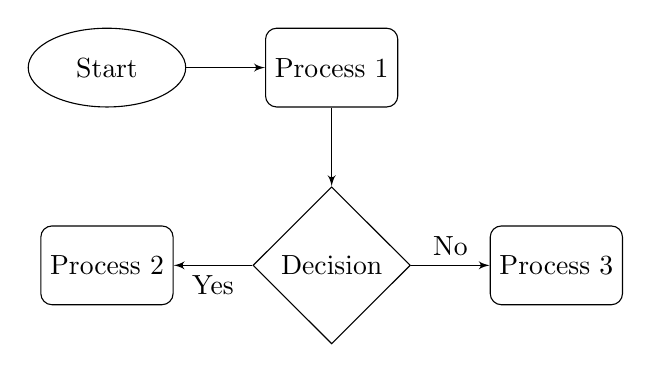
\begin{tikzpicture}[node distance=1cm, auto]
		\node [goal] (start) {Start};
		\node [process, right=of start] (proc1) {Process 1};
		\node [decision, below=of proc1] (yesno) {Decision};
		\node [process, left=of yesno] (proc2) {Process 2};
		\node [process, right=of yesno] (proc3) {Process 3};
	
		\path [line] (start) -- (proc1);
		\path [line] (proc1) -- (yesno);
		\path [line] (yesno) -- node {Yes} (proc2);
		\path [line] (yesno) -- node {No} (proc3);
	\end{tikzpicture}
\end{figure}

The following \LaTeX\space code produces the above figure:

\begin{lstlisting}[language=TeX]
\begin{figure}[h]
	\centering
	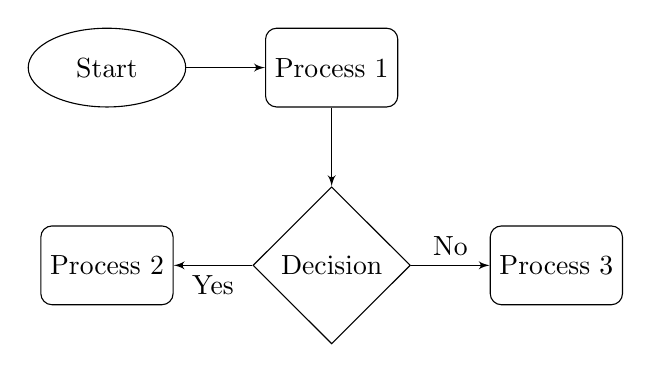
\begin{tikzpicture}[node distance=1cm, auto]
		\node [goal] (start) {Start};
		\node [process, right=of start] (proc1) {Process 1};
		\node [decision, below=of proc1] (yesno) {Decision};
		\node [process, left=of yesno] (proc2) {Process 2};
		\node [process, right=of yesno] (proc3) {Process 3};
	
		\path [line] (start) -- (proc1);
		\path [line] (proc1) -- (yesno);
		\path [line] (yesno) -- node {Yes} (proc2);
		\path [line] (yesno) -- node {No} (proc3);
	\end{tikzpicture}
\end{figure}
\end{lstlisting}

While this isn't a strict guide, there are some important things to note:

\begin{itemize}
	\item{The \texttt{figure} environment should have the \texttt{h}
		specifier to place the figure correctly in the page.}
	\item{The \texttt{tikzpicture} environment should have the
		\texttt{auto} and \texttt{node distance} specifiers set,
		with \texttt{node distance} kept to a reasonable size.}
	\item{The syntax for positioning nodes should be
		\texttt{[relative position]=of [node]} rather than
		\texttt{[relative position] of=[node]}. This is done so
		that the distance between nodes is properly respected.}
\end{itemize}

The only figure that shouldn't be included in an \texttt{figure} environment
is source code listings.

\section{Workshops}

Workshop exercises for this week go here.

\section{Exercises}

Solution to exercise sheets set this week go here.

\section{Labs}

Solutions to labs set this week go here.

\end{document}
